%-------------------------------------------------------------------------------
%                            BAB II
%               TINJAUAN PUSTAKA DAN DASAR TEORI
%-------------------------------------------------------------------------------
\fancyhf{} 
\fancyfoot[C]{\thepage}
\chapter{TINJAUAN KEPUSTAKAAN}               

\section{\uppercase{Hidroponik}}
Hidroponik merupakan cara budidaya tanaman dengan menggunakan air yang telah dilarutkan nutrisi yang dibutuhkan tanaman sebagai media tumbuh tanaman untuk menggantikan tanah. Konsentrasi larutan nutrisi harus dipertahankan pada tingkat tertentu agar pertumbuhan dan produksi tanaman optimal \citep{istiqomah2006menanam}. Hidroponik dapat menjadi salah satu alternatif terbatasnya lahan pertanian dan dapat dilakukan pada lahan yang kesuburannya rendah maupun wilayah padat penduduk. Komoditas yang dapat dipilih dalam budidaya secara hidroponik seperti \textit{endieve}, selada keriting hijau, selada keriting merah, \textit{lollo rossa, butterhead, christine, packcoy, monde} dan selada \textit{romaine} yang jarang dibudidayakan petani konvensional. Budidaya secara hidroponik lebih ramah lingkungan karena tidak menggunakan pestisida, tidak meninggalkan residu dan kebutuhan air lebih hemat serta tanaman tumbuh lebih cepat \citep{herwibowo2014hidroponik}.

\section{\uppercase{Pemasaran Digital}}
Pemasaran digital adalah suatu usaha untuk mempromosikan sebuah merek dengan menggunakan media digital yang dapat menjangkau konsumen secara tepat waktu, pribadi, dan relevan. Tipe pemasaran digital mencakup banyak teknik dan praktik yang terkandung dalam kategori pemasaran internet. Dengan adanya ketergantungan pemasaran tanpa internet membuat bidang pemasaran digital menggabungkan elemen utama lainnya seperti ponsel, SMS (pesan teks dikirim melalui ponsel), menampilkan iklan spanduk, dan digital luar. \citep{wikipedia2021}

\par Menurut \cite{tarigan2013creative} Pemasaran Digital adalah kegiatan pemasaran termasuk \textit{branding} yang menggunakan berbagai media berbasis web seperti blog, \textit{website}, \textit{e-mail}, \textit{adwords}, ataupun jejaring sosial. Tentu saja pemasaran digital bukan hanya berbicara tentang pemasaran internet.”

\section{\uppercase{E-commerce}}
Menurut \cite{yuhefizar2013} , “\textit{e-commerce} adalah singkatan dari \textit{electronic commerce}, yaitu sebuah layanan berbasis elektronik (internet) untuk bertransaksi/berdagang secara \textit{online}.” Sedangkan menurut \cite{saputra2013}, “\textit{e-commerce} adalah segala aktivitas transaksi produk ataupun jasa antara penjual dan pembeli dengan memanfaatkan kecanggihan elektronik, sehingga proses transaksi dapat dilakukan meskipun antara penjual dan pembeli tidak secara langsung bertatap muka.”

\section{\uppercase{Website}}
\textit{Website} adalah kumpulan dari beberapa halaman web dimana informasi dalam bentuk teks, gambar, suara, dan lain-lain dipresentasikan dalam bentuk \textit{hypertext} dan dapat diakses oleh perangkat lunak yang disebut dengan browser. Informasi pada sebuah \textit{website} pada umumnya di tulis dalam format HTML.

\par \textit{Website} merupakan fasilitas internet yang menghubungkan dokumen dalam lingkup lokal maupun jarak jauh. Dokumen pada \textit{website} disebut dengan web \textit{page} dan \textit{link} dalam \textit{website} memungkinkan pengguna bisa berpindah dari satu \textit{page} ke \textit{page} lain (\textit{hyper text}), baik diantara page yang disimpan dalam server yang sama maupun server diseluruh dunia. \textit{Pages} diakses dan dibaca melalui browser seperti Netscape Navigator atau Internet Exploler berbagai aplikasi browser lainnya. \citep{hakim2004}

\section{\uppercase{Entity Relationship Diagram (ERD)}}
Menurut \cite{priyadi2014} menyatakan bahwa : Pemodelan basis data dengan menggunakan diagram relasi antara entitas, dapat dilakukan dengan menggunakan suatu pemodelan basis data yang bernama Diagram \textit{Entity Relationship} yang disingkat Diagram E-R. ERD juga merupakan gambaran yang menghubungkan antara objek satu dengan objek yang lain dalam dunia nyata. Bisa dikatakan bahwa bahan yang akan digunakan untuk membuat ERD adalah dari objek di dunia nyata. Secara umum ERD terdiri dari 4 komponen, yakni :

\begin{enumerate}
	\item Entitas
	\par Entitas merupakan notasi untuk mewakili suatu objek dengan karakteristik sama, yang dilengkapi oleh atribut, sehingga pada suatu lingkungan nyata objek akan berbeda dengan objek lainnya.
	\item Relasi
	\par Relasi merupakan notasi yang digunakan untuk menghubungkan beberapa entitas berdasarkan fakta pada suatu lingkungan.
	\item Atribut
	\par Atribut merupakan notasi yang menjelaskan karakteristik suatu entitas dan juga relasinya. Atribut dapat sebagai \textit{key} yang bersifat unik, yaitu \textit{primary key} atau \textit{foreign key}. Selain itu, atribut juga dapat sebagai atribut deskriptif saja, yaitu sebagai pelengkap deskripsi suatu entitas dan relasi.	
	\item Garis Penghubung
	\par Garis penghubung merupakan notasi untuk merangkai keterkaitan antara notasi-notasi yang digunakan dalam Diagram E-R , yaitu entitas, Relasi , dan atribut.
\end{enumerate}

\section{\uppercase{Laravel Livewire}}
\par Laravel adalah sebuah \textit{Framework} PHP dirilis dibawah lisensi MIT dengan kode sumber yang sudah disediakan oleh GitHub, sama seperti \textit{framework-framework} yang lain, Laravel dibangun dengan konsep MVC \textit{(Model-View-Controller)}, kemudian Laravel dilengkapi juga \textit{command line tool} yang bernama “Artisan” yang bisa digunakan untuk \textit{packaging bundle} dan instalasi \textit{bundle} melalui \textit{command prompt} \citep{aminudin2015}.

\par Livewire adalah kerangka kerja \textit{full-stack} untuk kerangka Laravel yang membuat membangun antarmuka dinamis menjadi sederhana, tanpa meninggalkan kenyamanan Laravel. Jika Anda menggunakan Livewire dengan Laravel maka Anda tidak perlu khawatir tentang menulis kode Ajax jQuery, Livewire akan membantu menulis kode Ajax jQuery dengan cara yang sangat sederhana menggunakan PHP tanpa penyegaran halaman Validasi Laravel akan berfungsi, formulir akan dikirimkan, dll. Apa yang dilakukan Laravel Livewire? \citep{krishaweb2021}

\begin{itemize}
	\item Livewire merender \textit{output} komponen awal dengan halaman (seperti \textit{Blade} termasuk), dengan cara ini SEO \textit{friendly}.
	\item Ketika interaksi terjadi, Livewire membuat permintaan AJAX ke server dengan data yang diperbarui.
	\item Server merender ulang komponen dan merespons dengan HTML baru.
	\item Livewire kemudian dengan cerdas mengubah DOM sesuai dengan hal-hal yang berubah.
\end{itemize}

\begin{figure}[H]
\centering
{
\includegraphics [width = 10.5cm, height= 6cm]{gambar/laravel-livewire}}
\caption{Laravel Livewire \citep{krishaweb2021}}
\label{laravel_livewire}
\end{figure}

\section{\uppercase{MySQL}}
MySQL merupakan DBMS yang pertama kali mulai dikembangkan tahun 1994 oleh sebuah perusahaan software bernama TeD Data Konsult AB yang dikemudian hari berganti label menjadi MySQL-AB. Dewasa ini MySQL digunakan oleh sebagian besar web server yang ada di jagat internet. Disamping karena dianggap simpel, juga dapat di \textit{porting} pada berbagai sistem operasi sekelas server, seperti Windows, Linux, Solaris, Mac OS, BSD, Unix, IBM-AIX. \citep{fathansyah2012}.

\par Walaupun relative simple, MySQL memiliki fitur-fitur yang sangat baik, sehingga cocok untuk digunakan dalam implementasi aplikasi basis data, khususnya berbasis web. Setelah beberapa kali ganti pemilik, saat ini MySQL dimiliki oleh Oracle Corporation, sebuah perusahaan skala besar di bidang basis data \citep{fathansyah2012}.

\section{\uppercase{Web Service}}
Kasman mengemukakan, “\textit{Web Service} adalah aplikasi yang dibuat agar dapat dipanggil dan diakses oleh aplikasi lain melalui internet dengan menggunakan format pertukaran data sebagai format pengiriman pesan” \citep{kasman2015}. \cite{hartono2012pengaruh} mengungkapkan, “\textit{Web service} menyediakan standar komunikasi di antara berbagai aplikasi software yang berbeda-beda dan dapat berjalan di berbagai platform maupun framework. \textit{Web service} digunakan sebagai salah satu fasilitas yang disediakan oleh suatu web untuk menyediakan layanan dalam bentuk informasi kepada sistem lain, sehingga sistem lain dapat berinteraksi dengan sistem tersebut melalui layanan \textit{service} yang disediakan oleh suatu sistem yang menyediakan \textit{web service}.” 

\par \textit{Web service} sebenarnya adalah kumpulan dari fungsi dan \textit{method} yang terdapat pada server yang dapat dipanggil oleh klien dari jarak jauh kemudian untuk memanggil \textit{method-method} tersebut kita bebas menggunakan aplikasi yang akan dibuat dengan menggunakan Bahasa pemrograman apa saja yang dijalankan pada platform apa saja (Marthasari 2010, 2). Pada penelitian ini akan digunakan \textit{web services} dengan layanan protokol REST untuk membantu aplikasi penjualan tanaman hidroponik berbasis Android berinteraksi dengan \textit{database} yang terdapat di web server.

\section{\uppercase{REST}}
REST (\textit{Representational State Transfer}) merupakan standar arsitektur komunikasi berbasis web yang sering diterapkan dalam pengembangan layanan berbasis web. Umumnya menggunakan HTTP (\textit{Hypertext Transfer Protocol}) sebagai protokol untuk komunikasi data \citep{fielding2000architectural}. Pada arsitektur REST, REST server menyediakan \textit{resources} (sumber daya/data) dan REST \textit{client} mengakses dan menampilkan \textit{resource} tersebut untuk penggunaan selanjutnya. Setiap \textit{resource} diidentifikasi oleh URIs (\textit{Universal Resource Identifiers}) atau global ID. \textit{Resource} tersebut direpresentasikan dalam bentuk format teks, JSON atau XML. Pada umumnya formatnya menggunakan JSON dan XML.

\par Berikut metode HTTP yang umum digunakan dalam arsitektur berbasis REST:
\begin{enumerate}
	\item GET, menyediakan hanya akses baca pada \textit{resource}.
	\item PUT, digunakan untuk menciptakan \textit{resource} baru.
	\item DELETE, digunakan untuk menghapus \textit{resource}.
	\item POST, digunakan untuk memperbarui \textit{resource} yang ada atau membuat \textit{resource} baru.
	\item OPTIONS, digunakan untuk mendapatkan operasi yang di \textit{support} pada \textit{resource}.
\end{enumerate}

\section{\uppercase{Virtual Private Server (VPS)}}
\textit{Virtual Private Server} (VPS) adalah \textit{virtual machine} yang dijual sebagai layanan oleh \textit{hosting provider}, dalam VPS \textit{user} bisa mengakses dan mengelola seluruh aspek \textit{software} dari server termasuk akses administrator di sistem oprasi server sampai aplikasi yang akan di implementasikan di server tersebut. VPS dapat dibagi menjadi beberapa VM \textit{(Virtual Machines)}, dimana di setiap VM adalah berupa \textit{“Virtual server”} yang dapat di \textit{install} sistem operasi tersendiri. VPS terasa seperti sebuah \textit{Dedicated Server}. Dibanding dengan \textit{shared hosting}, menyewa VPS akan mendapatkan \textit{resource} yang lebih baik sehingga tidak terganggu jika ada problem pada \textit{website} yang dikelola. Selain itu VPS mendapatkan \textit{root} akses sehingga lebih leluasa dalam mengkustomasi server sesuai kebutuhan \citep{hamida2017analisis}.

\section{\uppercase{Scrum}}
Menurut \cite{pressman2010} \textit{scrum} adalah metode pengembangan peranti lunak secara cepat (\textit{agile}). Prinsip \textit{scrum} sesuai dengan prinsip-prinsip yang terdapat pada metode pengembangan peranti secara cepat yang digunakan untuk menuntun kegiatan pengembangan peranti lunak, seperti: pemenuhan kebutuhan, analisa, desain, dan penyampaian (\textit{delivery}). Alur proses \textit{scrum} dapat dilihat pada gambar 2.1 : 

\begin{figure}[H]
\centering
{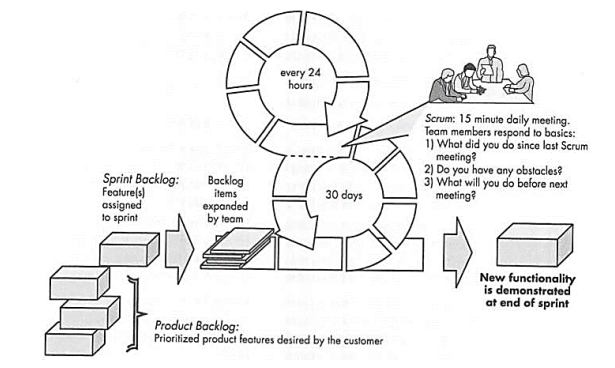
\includegraphics [width = 12.5cm, height= 8cm]{gambar/alur_proses_scrum}}
\caption{Alur Proses Scrum \citep{pressman2010}}
\label{alur_proses_scrum}
\end{figure}	

\par Menurut \cite{pressman2010}, di setiap tahap pengembangan, terjadi aktivitas kerja yang terlingkup di dalam suatu pola proses yang dinamakan sprint. Setiap pola proses yang terjadi, akan terdapat seperangkat kegiatan berikut: 

\begin{enumerate}[a.]
\item \textit{Backlog}
 \par Sebuah rincian prioritas pada fitur-fitur yang akan dibangun pada suatu proyek. Isi pada fitur dapat ditambahkan setiap saat. 
 \item \textit{Sprints} 
 \par Kumpulan aktivitas kerja yang dilakukan untuk memenuhi kebutuhan yang ditetapkan dalam \textit{backlog} dan harus diselesaikan pada waktu yang telah ditentukan. Perubahan tidak dapat dilakukan pada proses sprint sehingga setiap tim akan bekerja di dalam lingkungan yang stabil. 
 \item \textit{Scrum Meeting} 
 \par Pertemuan yang dilakukan setiap hari oleh tim \textit{scrum} untuk membahas apa yang telah dikerjakan sejak pertemuan terakhir, merencanakan dan membahas masalah-masalah yang ada (biasanya 15 menit).
 \item \textit{Demos} 
 \par Menujukan hasil fungsionalitas yang telah diimplementasikan sehingga dapat dievaluasi oleh pengguna. 
 Demo harus berupa fitur-fitur yang telah diselesaikan sesuai dengan waktu yang telah ditetapkan. 
\end{enumerate}

\section{\uppercase{Black Box Testing}}
Pengujian \textit{black box (black box testing)} adalah salah satu metode pengujian perangkat lunak yang berfokus pada sisi fungsionalitas, khususnya pada \textit{input} dan \textit{output} aplikasi (apakah sudah sesuai dengan apa yang diharapkan atau belum). Tahap pengujian atau testing merupakan salah satu tahap yang harus ada dalam sebuah siklus pengembangan perangkat lunak (selain tahap perancangan atau desain) \citep{iskandaria2012}. Menurut \cite{shihab2011} kategori kesalahan/\textit{error} yang akan diketahui melalui \textit{black box} testing :

\begin{itemize}
\item Fungsi yang hilang atau tak benar/salah
\item \textit{Error} dari antar-muka/\textit{interface}
\item \textit{Error} dari struktur data atau akses eksternal \textit{database}
\item \textit{Error} dari kinerja atau tingkah laku/\textit{perform}
\item \textit{Error} dari inisialisasi dan terminasi
\end{itemize}


\section{\uppercase{System Usability Scale (SUS)}}
\textit{System Usability Scale} adalah sebuah metode uji pengguna yang digunakan untuk mengukur \textit{usability}. John Brooke mengembangkan \textit{System Usability Scale} pada tahun 1986 sebagai metode yang menyediakan alat ukur bersifat \textit{“quick and dirty”}. Menurut Brooke, \textit{System Usability Scale} memungkinkan untuk mengevaluasi berbagai macam produk dan jasa, termasuk \textit{hardware, software, website} dan aplikasi. 

\par Metode penilaian \textit{System Usability Scale} mengharuskan para peserta untuk memberikan tanggapan terhadap 10 item pernyataan menggunakan 5 poin skala \textit{Likert}. Responden diminta untuk memberikan penilaian dari skala 1 yang berarti “Sangat tidak setuju”, skala 2 yang berarti “Tidak setuju”, skala 3 yang berarti “Netral”, skala 4 yang berarti “Setuju”, dan skala 5 yang berarti “Sangat setuju”. Jika karena alasan tertentu, Jika responden merasa tidak menemukan skala respon yang tepat, responden harus mengisi titik tengah skala pengujian. \textit{System Usability Scale} dipercaya skala yang dapat digunakan untuk dua faktor yang berbeda, yaitu mengukur keseluruhan dari \textit{usability} (8 dari 10 item) dan mengukur \textit{learnability} 
(2 dari 10 item) dari suatu sistem. 

\par Adapun 10 item pertanyaan kuesioner yang digunakan dalam metode ini :

\begin{table}[H]
\centering
\caption{Item Pernyataan \textit{System Usability Scale} \citep{bangor2008, finstad2006}}
\label{item_pernyataan_system_usability_scale}
\begin{tabular}{|l| >{\centering\arraybackslash} m{10cm}| >{\centering\arraybackslash} m{2cm}|} 
\hline
\textbf{No.} & \textbf{Pernyataan} & \textbf{Skala}  \\ 
\hline
1.           & Saya pikir bahwa saya akan ingin lebih sering menggunakan aplikasi ini      & 1 s/d 5   \\ 
\hline
2.           & Saya merasa sistem ini tidak harus dibuat serumit ini		& 1 s/d 5  \\ 
\hline
3.           & Saya pikir sistem ini mudah digunakan     		& 1 s/d 5   \\ 
\hline
4.           & Saya pikir saya perlu bantuan tenaga teknis agar dapat menggunakan sistem ini      		& 1 s/d 5      \\ 
\hline
5.           & Saya menemukan berbagai fungsi pada sistem ini terintegrasikan dengan baik        	& 1 s/d 5   \\
\hline
6.           & Saya pikir ada terlalu banyak ketidaksesuaian dalam sistem ini   & 1 s/d 5   \\
\hline
7.           & Saya bayangkan bahwa kebanyakan orang akan belajar menggunakan sistem dengan cepat    & 1 s/d 5   \\
\hline
8.           & Saya menemukan bahwa sistem sangat rumit digunakan   & 1 s/d 5   \\
\hline
9.           & Saya merasa sangat percaya diri untuk menggunakan sistem ini   & 1 s/d 5   \\
\hline
10.           & Saya perlu belajar banyak hal sebelum saya bisa 
menggunakan sistem ini   & 1 s/d 5   \\
\hline
\end{tabular}
\end{table}

%-----------------------------------------------------------------------------%

% Baris ini digunakan untuk membantu dalam melakukan sitasi
% Karena diapit dengan comment, maka baris ini akan diabaikan
% oleh compiler LaTeX.

\fancyhf{} 
\fancyfoot[R]{\thepage}

\begin{comment}
\bibliography{daftar-pustaka}
\end{comment}
